\normaltrue \difficilefalse \tdifficilefalse
\correctionfalse

%\UPSTIidClasse{11} % 11 sup, 12 spé
%\newcommand{\UPSTIidClasse}{12}

\exer{Cylindre percé $\star$ \label{B2:10:42}}
\setcounter{numques}{0}
\UPSTIcompetence[2]{B2-10}
\index{Compétence B2-10}
\index{Parallélépipède}
\ifcorrection
\else
\textbf{Pas de corrigé pour cet exercice.}
\fi

\ifprof
\else

La matrice d'inertie d'un cylindre d'axe $\axe{G}{k}$ de rayon $R$ et de hauteur $H$ et de masse $m$ est donnée en son centre d'inertie par 
$\inertie{G}{1}=\matinertie{A}{A}{C}{0}{0}{0}{\base{i}{j}{k}}$ avec $A=m\left(\dfrac{R^2}{4}+\dfrac{H^2}{12} \right)$ et $C=m\dfrac{R^2}{2}$. 


Soit la pièce suivante. 
\begin{figure}[H]
\centering
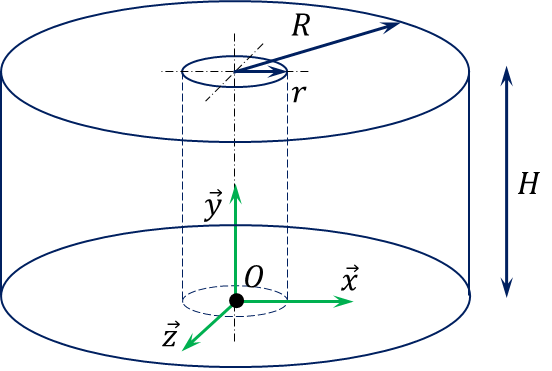
\includegraphics[width=.7\linewidth]{42_01}
\end{figure}

On pose $\vect{OA}=-\dfrac{R}{2}\vect{x}$.

\fi


\question{Déterminer la position du centre d'inertie $G$ du solide.}
\ifprof
\else
\fi

\question{Déterminer la matrice d'inertie du solide en $G$ puis en $O$.}
\ifprof ~\\
\else
\fi


\ifprof
\else
\begin{flushright}
\footnotesize{Corrigé voir \ref{B2:10:42}.}
\end{flushright}%
\fi